\documentclass[revision-guide.tex]{subfiles}
%% Current Author:
\setcounter{chapter}{8}
\begin{document}
\tikzset{component/.style={draw,thick,circle,fill=white,minimum size =0.75    cm,inner sep=0pt}}
\chapter{Quantum Ideas}
\begin{content}
  \item the photoelectric effect
  \item the photon
  \item wave-particle duality
\end{content}
\section*{Candidates should be able to:}

\spec{recall that, for monochromatic light, the number of photoelectrons emitted per second is proportional to the light intensity and that emission occurs instantaneously}

\spec{recall that the kinetic energy of photoelectrons varies from zero to a maximum, and that the maximum kinetic energy depends on the frequency of the light, but not on its intensity}

\spec{recall that photoelectrons are not ejected when the light has a frequency lower than a certain threshold frequency which varies from metal to metal}

\rule{\textwidth}{0.1pt}

\spec{understand how the wave description of light fails to account for the observed features of the photoelectric effect and that the photon description is needed}

Each of the above features \emph{(a) - (c)} is discussed in turn below.

\begin{enumerate}[label=\emph{(\alph*)}]
\item In the wave description of light the energy an electron in the metal receives energy from the light arrives continuously. An electron  therefore gradually absorbs enough energy to escape from the surface of the metal, something which is not seen in practice. Additionally, increasing the intensity of a wave corresponds to increasing the amplitude of the oscillation. This would lead us to expect that increasing the intensity of light would give photoelectrons of a higher energy, rather than simply more of them.

The photon description of light accounts of both of these effects. When light arrives on the surface of the metal a single photon interacts with a single electron. Assuming the photon gives the electron enough energy to escape, the electron will leave the metal instantaneously. In the photon model, the intensity of the light is due to the number of photons arriving per second. Therefore if the intensity doubles, the number of photons doubles and the number of photoelectrons doubles.

\item When the photoelectrons leave the metal some of the photon energy is used to break away from the metal and the remainder goes into their kinetic energy. Different photoelectrons have different amounts of energy, however there is a maximum kinetic energy the photoelectrons are found to have and this depends \emph{only} on the frequency of the incoming radiation.

The wave model of light would allow different electrons to absorb different amounts of energy and therefore this relationship would not be seen.

\item The energy from a photon of light is split between the energy required to escape the metal and the kinetic energy of the photoelectron. If the photon does not have enough energy to enable to the electron to escape the metal then no emission of photoelectrons is seen.

The wave model would still allow emission as a single electron could absorb energy from the wave over a longer period of time. However, since there are so many electrons in the surface of the metal it is vanishingly unlikely that a single photoelectron will interact with two photons.

\end{enumerate}

\spec{recall that the absorption of a photon of energy can result in the emission of a photoelectron}

As described above.

\spec{recognise and use $E = hf$}

The energy of a photon of light is related to the frequency of that radiation using the equation $E=hf$ where $h$ is Planck's Constant which has a value of \SI{6.626e-34}{\joule\second}.

\spec{understand and use the terms threshold frequency and work function and recall and use
\begin{equation}\label{eqn:photoelectric}
hf = \phi + \frac{1}{2}mv_{\text{max}}^2
\end{equation}}

\begin{description}
  \item[Threshold Frequency, $f_0$.] This is the minimum frequency required for the emission of photoelectrons to occur. This varies from metal to metal.
  \item[Work Function, $\phi$.] This is the energy required to remove an electron from the surface of the metal.
\end{description}

Equation \ref{eqn:photoelectric} expresses the sharing of the energy of the photon ($hf$) between the work function ($\phi$) and the kinetic energy of the photoelectron.

\spec{understand the use of stopping potential to find the maximum kinetic energy of photoelectrons and convert energies between joules and electron-volts}

We can measure the energy of the photoelectrons by placing a photocell in a circuit and using a potential difference to stop the flow of electrons.

\begin{figure}[h]
\begin{center}
\begin{circuitikz}
  \draw (5,0) -- (5,3) to[pvsource] (0,3);
  \draw (0,0) -- (0,1.5) node[component]{\si{\micro\ampere}} --(0,3);
  \draw (5,0) to[battery] (0,0);
  \draw (1,0) -- (1, -1.5) -- (2.5,-1.5) node[component]{V} -- (4,-1.5) -- (4,0);
  \draw[->] (2.1,-0.5) -- (2.9,0.5);
\end{circuitikz}
\end{center}
\caption{Measuring stopping potential}
\label{fig:stopping-pot}
\end{figure}

Figure \ref{fig:stopping-pot} shows a simple set-up to measure the stopping potential for photoelectrons. Monochromatic light is shone on the photocell. Electrons leave the surface of the metal and travel around the circuit creating a small current. The variable power supply is gradually increased until no current flows through the circuit. At this point none of the electrons leaving the surface of the metal in the photocell have enough energy to cross the potential difference and create a current in the circuit. At this point the maximum energy of the photoelectrons can be equated to the energy required to cross a potential difference $V$:
\begin{equation}\label{eqn:photoelectron-stopping-pot}
  \frac{1}{2}mv_{\text{max}}^2 = eV
\end{equation}

Since we are measuring the energies of electrons using potential differences, it makes sense to define a unit of energy in terms of these potential differences. Hence, 1 electronvolt is defined as the energy transferred by an electron moving through a potential difference of 1 volt.
\begin{equation}
  \SI{1}{\electronvolt} = \SI{1.6e-19}{\joule}
\end{equation}

\spec{plot a graph of stopping potential against frequency to determine the Planck constant, work function and threshold frequency}

By repeating the experiment shown in Figure \ref{fig:stopping-pot} for different frequencies of light and measuring the stopping potential for each frequency we get the graph shown in Figure \ref{fig:milikan-results}.

\begin{figure}[ht]
  \begin{center}
    \begin{tikzpicture}
      \draw[<->] (0,5) node[anchor=north east, align=right]{stopping\\potential\\/ \si{\volt}} -- (0,0) -- (7,0) node[anchor=north,align=left]{frequency\\/ \si{\hertz}};
      \draw[thick] (2,0) node[anchor=north, align=left]{threshold\\frequency,\\$f_0$} -- (6.5,4.5);
    \end{tikzpicture}
  \end{center}
  \caption{Stopping potential against threshold frequency}
  \label{fig:milikan-results}
\end{figure}

Equation \ref{eqn:photoelectric} and \ref{eqn:photoelectron-stopping-pot} can be combined with  and re-arranged to give
\begin{equation}\label{eqn:milikan}
V = \frac{h}{e}f - \frac{\phi}{e}
\end{equation}

Equation \ref{eqn:milikan} describes the linear relation seen on the graph in Figure \ref{fig:milikan-results}. The graph has a gradient of $\frac{h}{e}$ which enables the determination of the Planck Constant and the intercept with the x-axis gives the threshold frequency. The work function is simply the energy of a photon with the threshold frequency, i.e.
\begin{equation}
  \phi = hf_0
\end{equation}

\spec{understand the need for a wave model to explain electron diffraction}

When electrons are fired at two closely spaced slits the result is entirely unlike what one would expect from a particle model. A particle model would predict that each electron would either go through one slit or the other, creating two regions at which electrons are found as shown in Figure \ref{fig:electron-diff-expected}.

\begin{figure}[h]
  \begin{center}
    \begin{tikzpicture}[scale=0.7]
      \usetikzlibrary{fadings}
      \draw (0,0) rectangle (1.5,3);
      \draw (1.7,0) rectangle (2.7,3);
      \draw (2.9,0) rectangle (4.4,3);
      \filldraw[fill=black!40!white] (3.5,3.7) rectangle (7.5,6.7);
      \draw[rotate around={-40:(-0,-1)}] (0,-1.5) rectangle (.4,-.5);
      \fill[pattern=crosshatch dots, pattern color=white] (4.5,5.2) circle [x radius=0.4, y radius=1.5];
      \fill[pattern=crosshatch dots, pattern color=white] (6.5,5.2) circle [x radius=0.4, y radius=1.5];
    \end{tikzpicture}
  \end{center}
  \caption{Expected pattern for electron diffraction}
  \label{fig:electron-diff-expected}
\end{figure}


However, this behaviour is not seen but rather electrons form an interference pattern similar to that seen for light, as shown in Figure \ref{fig:electron-diff-observed}.

\begin{figure}[!h]
  \begin{center}
    \begin{tikzpicture}[scale=0.7]
      \usetikzlibrary{fadings}
      \draw (0,0) rectangle (1.5,3);
      \draw (1.7,0) rectangle (2.7,3);
      \draw (2.9,0) rectangle (4.4,3);
      \filldraw[fill=black!40!white] (3.5,3.7) rectangle (7.5,6.7);
      \draw[rotate around={-40:(-0,-1)}] (0,-1.5) rectangle (.4,-.5);
      \foreach \x in {4,4.5,...,7} {
        \fill[pattern=crosshatch dots, pattern color=white] (\x,5.2) circle [x radius=0.15, y radius=1.5];
      }
    \end{tikzpicture}
  \end{center}
  \caption{Observed pattern for electron diffraction}
  \label{fig:electron-diff-observed}
\end{figure}

The mystery here is how can single particles form an interference pattern? If electrons are fired through two slits one at a time then they initially appear to arrive randomly. As more and more arrive they fill in the interference pattern. We explain this by saying that the probability of their arrival is determined by a form of wave-mechanics and as particles arrive they fill in the probability pattern as shown in figure \ref{fig:electron-buildup}.

\begin{figure}
  \begin{center}
  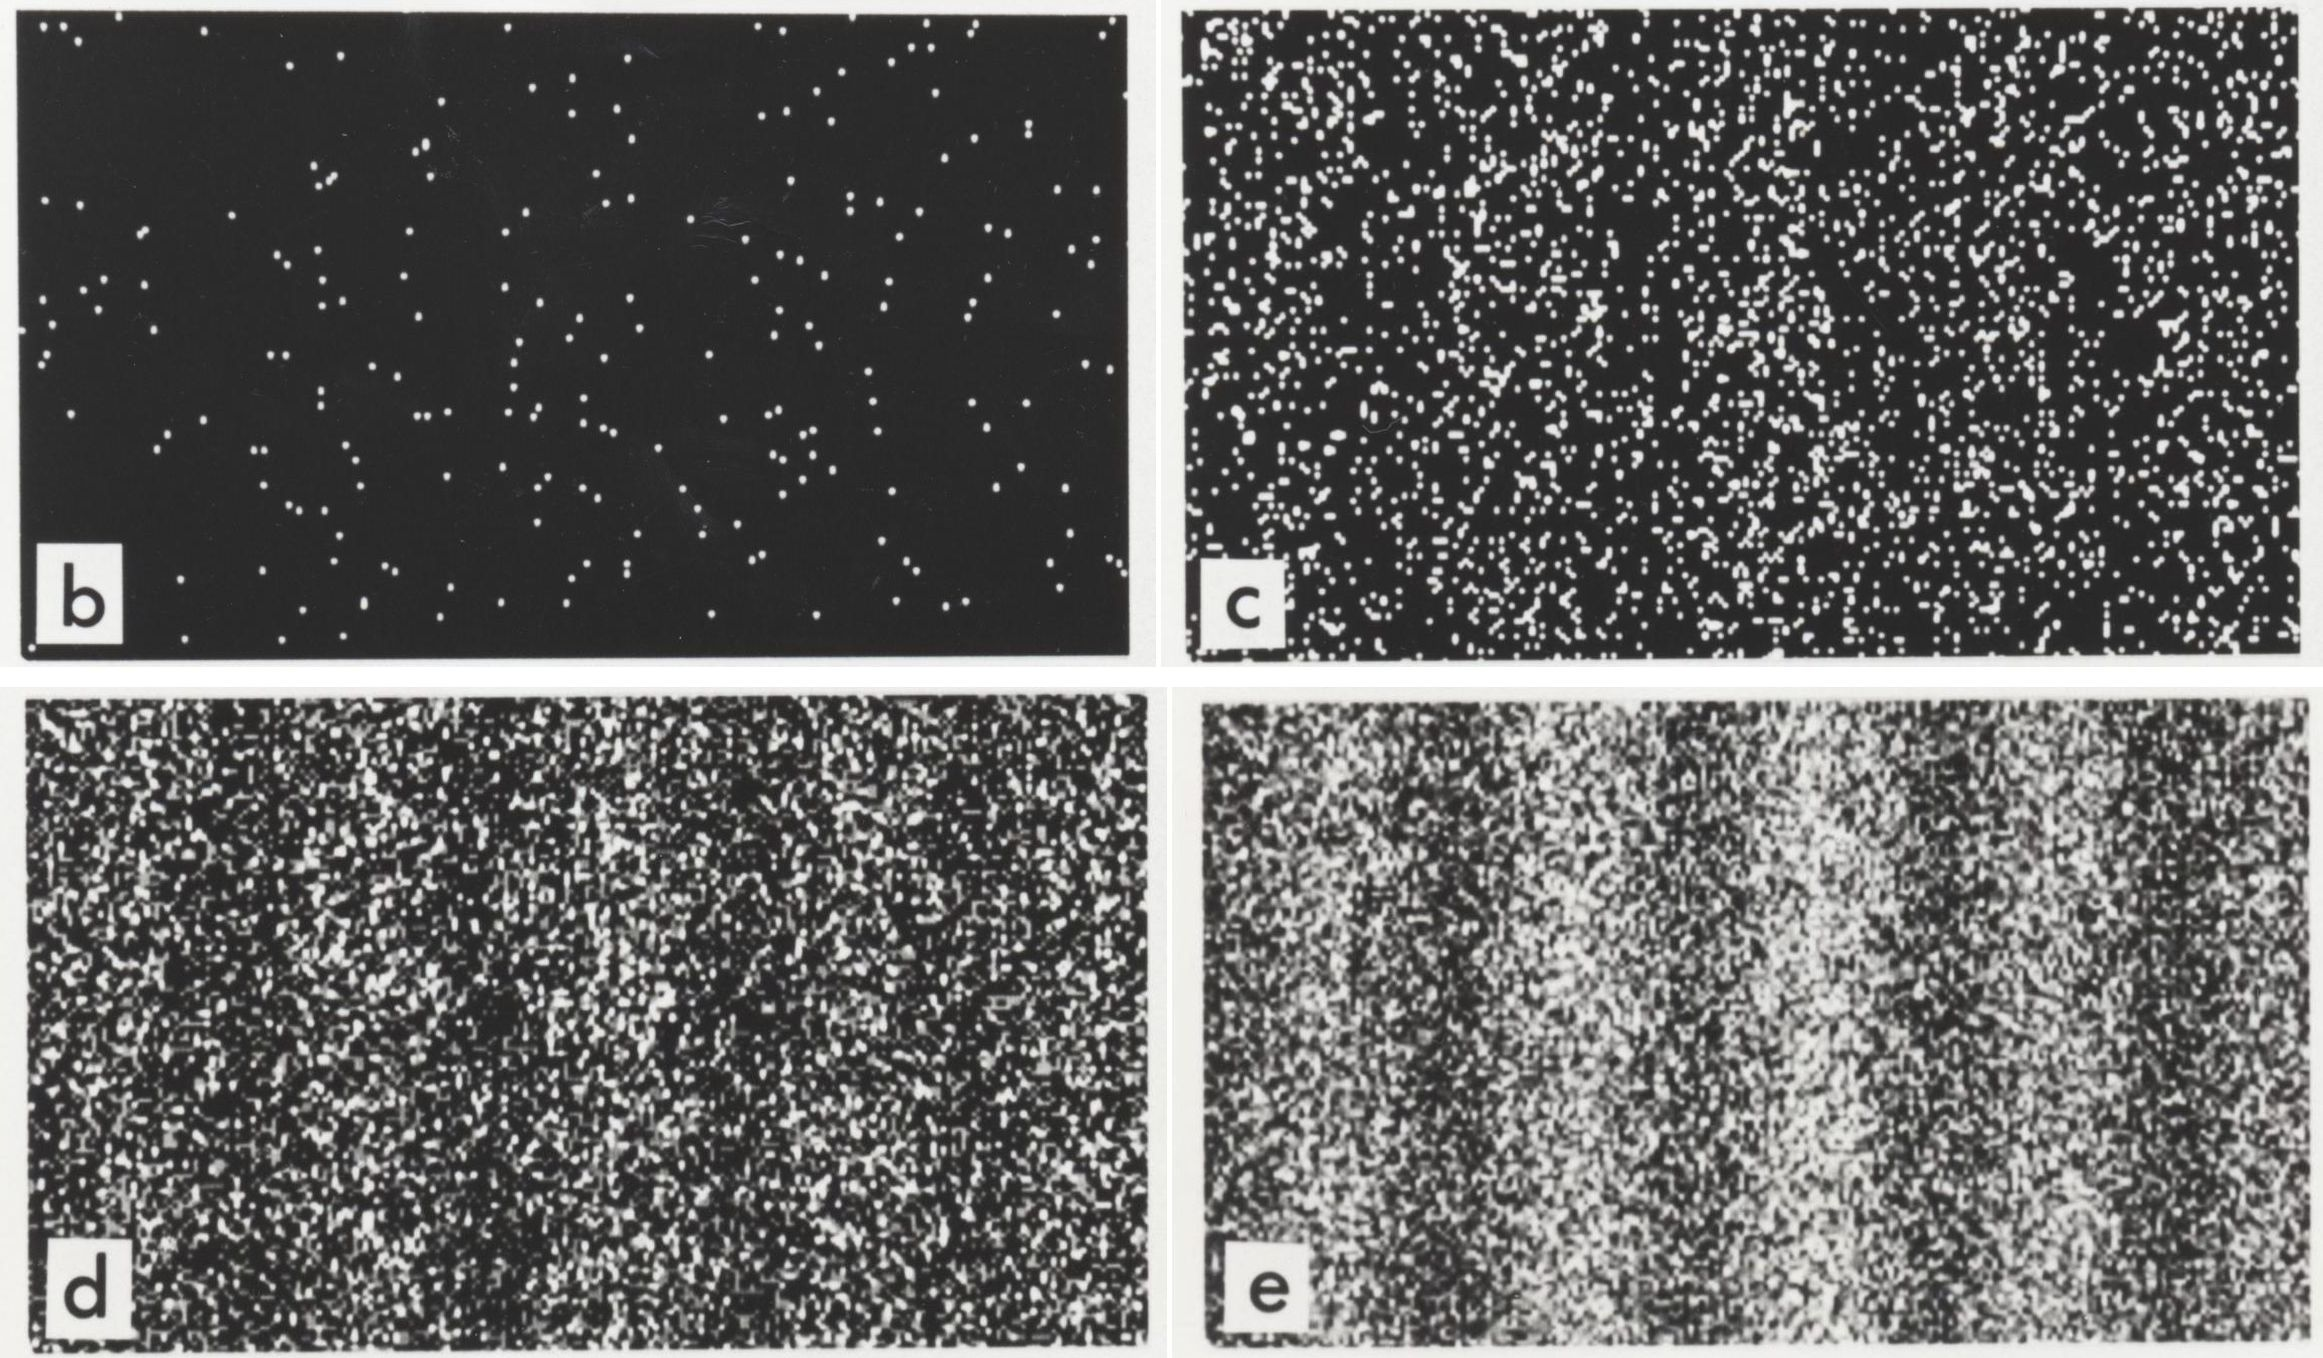
\includegraphics[width=0.8\textwidth]{figs/chapt-9/electron-diff.jpg}
\end{center}
  \caption{Build up of the interference pattern of electrons. \emph{Credit: Belsazar, Wikimedia Commons}}
  \label{fig:electron-buildup}
\end{figure}

\clearpage

\spec{recognise and use
\begin{equation}\label{eqn:debroglie}
\lambda = \frac{h}{p}
\end{equation} for the de Broglie wavelength.}

In order to explain the wave-like nature of electrons we need to be able to assign them a wavelength. de Broglie's thesis is that \emph{all} particles have a wavelength which is defined in equation \ref{eqn:debroglie}. This brings wave-particle duality from photons and electrons to all particles. The natural question here is why isn't interference ordinarily observed? The answer is that the de Broglie wavelength for macroscopic objects is extremely small and therefore these objects behave as particles, travelling in straight lines and not undergoing interference.

\begin{example}
Electrons will be diffracted by crystal lattices if they have a wavelength of around \SI{0.1}{\nano\metre}. Calculate the speed and energy of such electrons.

\answer
The speed of these electrons can therefore be calculated as follows:
\[ \lambda = \frac{h}{p} = \frac{h}{mv} \]
\[ v = \frac{h}{m\lambda} = \SI{7.27e6}{\meter\per\second} \]
\[ E = \frac{1}{2}mv^2 = \SI{151}{\electronvolt} \]

\end{example}
\end{document}
